\documentclass[a4paper]{article}
\usepackage[bottom=10em]{geometry}

\usepackage[T1]{fontenc}	
\usepackage{amsmath}
\usepackage{amssymb}
\usepackage{graphicx}
\usepackage{fancyhdr}
\usepackage{array}
\usepackage{float}
\usepackage{booktabs}


\pagestyle{fancy}
\lhead{Computer Excercise 2}
\rhead{Kristoffer Nordström \& Noah Hansson}

\title{Computer Exercise 2 - NEKN83}
\author{Kristoffer Nordström \& Noah Hansson}
\date{\today}

\setlength{\parskip}{0.7em}
\setlength{\parindent}{0pt}
\setlength{\floatsep}{6pt plus 1.0pt minus 2.0pt}
\setlength{\textfloatsep}{10pt plus 1.0pt minus 2.0pt}

\begin{document}

\maketitle


\section{Introduction}
In this computer exercise the aim is to implement, evaluate and compare different methods for estimating the Expected Shortfall\footnote{Henceforth referred to as ES} for the US stock market index SP500.

\section{Method}
The data used for this exercise is the daily recorded returns of the SP500 market index during the years 2013 - 2015. The returns are then converted to losses by assuming that we hold a portfolio of \$1000 each day. We will then use this data to evaluate Value-at-Risk\footnote{Henceforth referred to as VaR}, and then the ES, using different assumptions and implementations. The ES estimate will be accepted or rejected using the Acerbi \& Szekely Z-test statistic with a 95\% confidence level as well as a Basel-type traffic light system. The Trafic light system will also be used to evaluate the VaR estimates. The VaR and ES will estimated in five different ways:
\begin{itemize}
    \item Normal
    \item Normal-EWMA
    \item T-dist
    \item T-dist EWMA
    \item Basic Historical Simulation
\end{itemize}
Through the whole computer exercise the certainty level for VaR and ES will be 97.5\%. 

All data and calculations are handled in Microsoft Excel, and the plots are generated in Python.

\section{Results}
\begin{table}[H]
    \centering
    \caption{ES performance measured in Z-test and Traffic Light results}
    \vspace{0.2cm}
    \begin{tabular}{lrrr}
        \toprule
                Model &  Z (test stat.) & Accept/Reject & Traffic Light \\
        \midrule
                Normal &       -1.742215 &        Reject &                         Yellow \\
            Normal-EWMA &       -0.727824 &        Reject &                         Yellow \\
                T-dist &       -1.203534 &        Reject &                         Yellow \\
            T-dist-EWMA &       -0.628559 &        Accept &                          Green \\
            BHS &       -1.000707 &        Reject &                         Yellow \\
        \bottomrule
    \end{tabular} 
\end{table}



\begin{table}[H]
    \centering
    \caption{VaR performance measured in number of violations and Traffic Light results}
    \vspace{0.2cm}
    \begin{tabular}{lrr}
        \toprule
              Model &  VaR Violations & Traffic Light \\
        \midrule
              Normal &               14 &                           Yellow \\
         Normal-EWMA &                9 &                            Green \\
              T-dist &               11 &                           Yellow \\
         T-dist-EWMA &                9 &                            Green \\
            BHS &               11 &                           Yellow \\
        \bottomrule
    \end{tabular}    
\end{table}
 
\begin{figure}[h]
    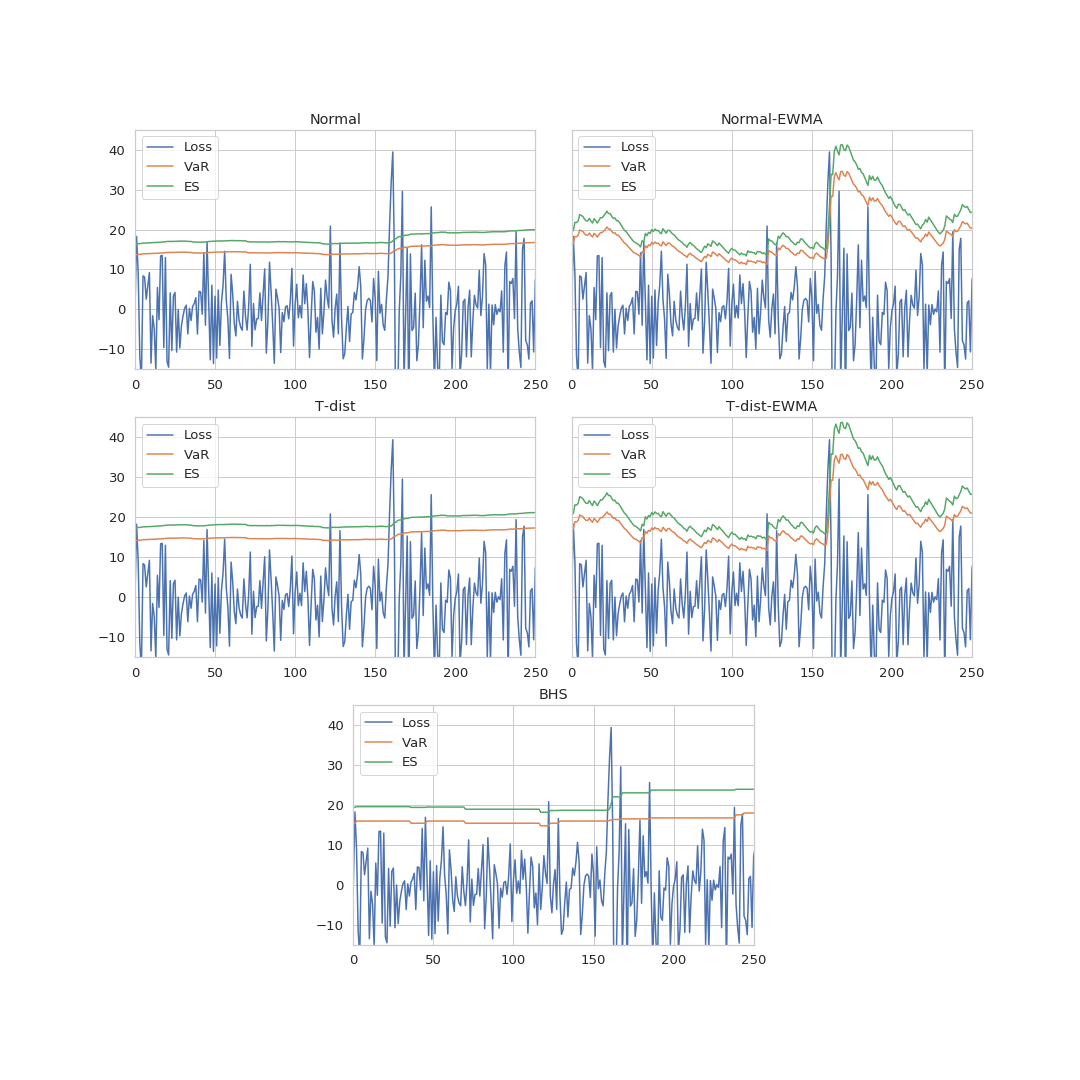
\includegraphics[width=\textwidth]{plot.png}
    \caption{$VaR_{97.5\%}$ (Orange) and $ES_{97.5\%}$ (Green) compared to Loss (Blue) for each day during the test period}
    \label{var2}
\end{figure}

\section{Conclusion}
The only method that passed the 95\% confidence Kupiec Test for estimating VaR in Exercise 1 was the T-EWMA-method. The same method scored green both when estimating ES and VaR in this exercise. The N-EWMA scored green on estimating the VaR between 2013-2015 and was just outside the confidence interval in the first exercise. 

When looking at the plotted VaR and ES we can see that the same conclusions that could be made for VaR in computer exercise 1 can be made for ES in this exercise. That is, the underlying assumptions of the loss distribution are not as important as finding a good way to describe the volatility of the asset. 
\end{document}